%!TEX root = ../report.tex
\chapter{Feature extraction} % (fold)
\label{chap:feature_extraction}
The goal of this chapter is to explain how the target object is detected in both images. With these positions the stereopsis can be computed as explained in chapter \ref{chap:stereopsis} and hence the 3D position of the target in the world can be obtained.
The tracking of the object is a function implemented inside the node "balltracker" explained in chapter \ref{chap:ros_nodes_structure}.

\section{Methods}

\subsection{Target definition}
The underlying problem of the feature extraction is providing a feature strong enough that avoids correspondence problems such as occluding edges, homogeneous areas and repetitive structures.
In the case of occluding edges, the main problem is that a feature in the border of the object for one camera usually matches another one from the other camera (specially for round or cylindrical objects) although they are not the same point.
On the other hand, the problem with homogeneous areas is that all the patches of a smooth surface with a constant illumination look exactly the same and can be mismatched.
Finally, the problem of repetitive surfaces affects mainly when it comes to matching images containing structures like fences or buildings which are usually very repetitive and can lead to mismatch features because they look too similar.
To avoid these problems, it was decided to use a ball as the target object.
The reason for this is that the whole area of the surface of the ball can be seen by each camera and, hence, its centroid detected, completely avoiding the occluding edges and the homogeneous surfaces. What is more, the ball itself is not a repetitive structure, so that doesn't produce a problem either.

\subsection{Image processing}
To achieve a reliable detection of the target in both images it was decided to use the contour finder provided by OpenCV.
For doing so a binary image is needed as an input for the contour finder as this function uses the algorithm in \cite{suzuki}. 
The binary image is obtained by first converting the input image from RGB to HSV colorspace.
The reason for this is that the last one provides an easier way of tracking colours more complex than the pure red, green or blue.
Then, the proper values for the hue, saturation and value are obtained by trial and error and then the 3 channels are thresholded, producing binary image that can be seen in figure \ref{fig:binary_image}.
However, this process yields some artefacts in the image that need to be removed for the contour finder not to detect too many unnecessary contours.
 
\begin{figure}[!ht]
    \centering
    %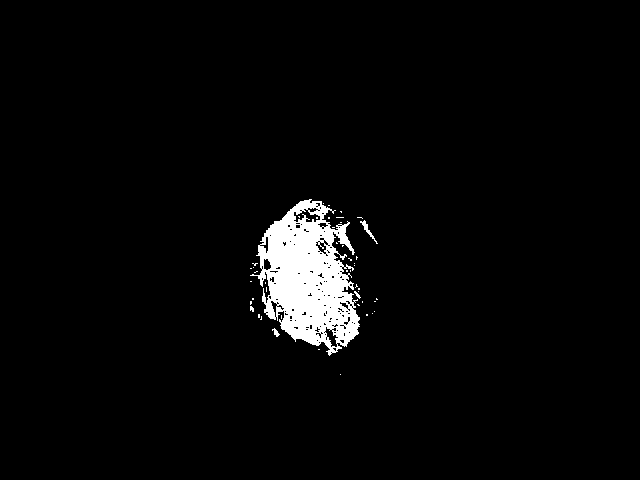
\includegraphics[width=0.8\textwidth]{images/binary.png}
    \caption{Binary image obtained after applying color threshold}
    \label{fig:binary_image}
\end{figure}

For removing those artefacts two morphological operators are applied. First of all an opening operation with a square kernel of 9x9 pixels that removes the small artefacts spread across the image and keeps the target intact. After this, a closing operation is perform with the same kernel. In this case, the aim of this is reducing the size of the gaps that appear inside the target after the thresholding in order to get a solid object. The result of this process can be seen in figure \ref{fig:filtered_image}.

\begin{figure}[h]
    \centering
    %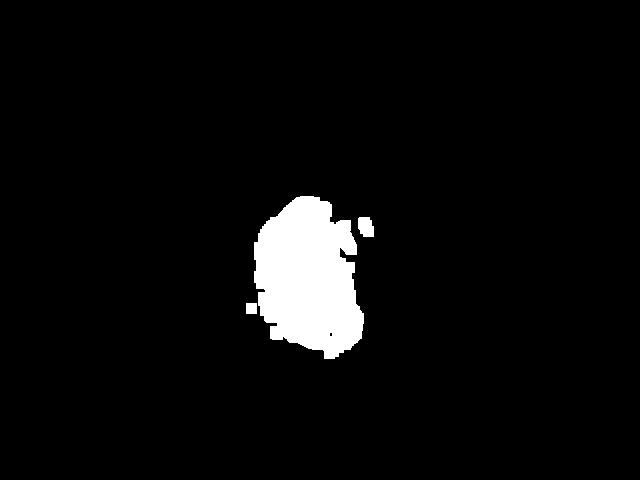
\includegraphics[width=0.8\textwidth]{images/filtered.png}
    \caption{Binary image obtained after applying the morphological operations}
    \label{fig:filtered_image}
\end{figure}

After removing the smallest objects from the binary image and closed the gaps in the remaining ones the finding contours function is applied, which provides an array with the detected contours. Following, the area and the outer perimeter of all the contours are computed. With these values, a radius threshold is applied so that only the contours with enough radius are accepted. For doing so, the equations for the perimeter and the area of a circumference are applied as it can be seen in equations \ref{eq:circ_perimeter} and \ref{eq:circ_area}.

\begin{equation}
perimeter_{contour}>2*\pi*radius_{threshold}
\label{eq:circ_perimeter}
\end{equation}

\begin{equation}
area_{contour}>2*\pi*radius_{threshold}^{2}
\label{eq:circ_area}
\end{equation}

Following, the circularity of the contours that have a radius bigger than the specified threshold is computed following equation \ref{eq:circularity}, which gives a value between 1 and 0 (being 1 a perfect circle, and 0 a straight line). Having this value computed, a threshold for the circularity is set so that only the target passes it. Finally, the moments of the remaining contour (the target) are calculated so that the centroids can be computed according to equation \ref{eq:centroids}. Then, this values are returned so that the stereopsis function can compute the 3D points for the target.

\begin{equation}
circularity=\frac{4*\pi*area_{contour}}{perimeter_{contour}^{2}}
\label{eq:circularity}
\end{equation}

\begin{equation}
centroid_{X}=\frac{m_{10}}{m_{00}} \qquad centroid_{Y}=\frac{m_{01}}{m_{00}}
\label{eq:centroids}
\end{equation}

\section{Results}
Several variations of the algorithm stated above were tested before ending up with that one. However, the original ball given as a marker to be tracked was completely white. Therefore, as the laboratory where the workcells are situated has high ceilings and the only windows are close to them, the sun was hitting with a high angle. 

This illumination configuration produced very bright spots on the top of the ball (easily seen by the cameras) while the rest of the ball stayed with less brightness. In addition, the walls surrounding the workcell are mainly white and, at certain moments of the day very bright. Consequently, tracking the white ball was a very difficult task. To fix this issue, the ball was covered with a piece of green paper that made the colour detection easier. Nevertheless, the high inclination of the sun still produced a spot of higher brightness in the top of the ball that wasn't detected by the algorithm. For fixing this, the closing morphology operation was performed as explained in the section above, which provided a much circular shape to the ball in the image than the one obtained by simply thresholding.

All in all, the final detection of the ball was stable enough to provide consistent data for the stereopsis and the trajectory prediction.

% chapter feature_extraction (end)~\ref{sec:}